\begin{frame}{Visualising the Clip}
\begin{center}
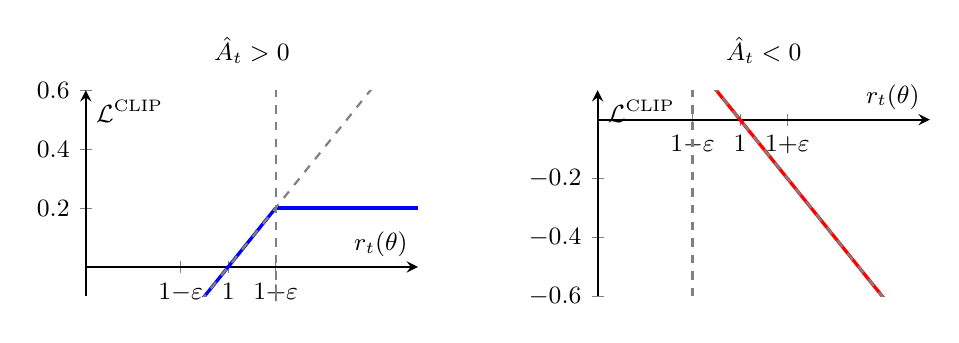
\begin{tikzpicture}
\pgfplotsset{
    width=5.8cm, height=4.2cm,
    axis lines=center,
    xlabel={$r_t(\theta)$},
    xtick={0.8,1,1.2},
    xticklabels={$1{-}\varepsilon$, $1$, $1{+}\varepsilon$},
    tick label style={font=\small},
    label style={font=\small},
    title style={font=\small\bfseries},
    xmin=0.4, xmax=1.8,
    every axis/.append style={thick}
}
% Left plot: A > 0
\begin{axis}[
    at={(0,0)},
    title={$\hat{A}_t > 0$},
    ylabel={$\mathcal{L}^{\mathrm{CLIP}}$},
    ymin=-0.1, ymax=0.6
]
\addplot[blue, very thick, domain=0.4:1.2] {x - 1};
\addplot[blue, very thick, domain=1.2:1.8] {0.2};
\addplot[dashed, gray, domain=0.4:1.8] {x - 1};
\draw[dashed, gray] (axis cs:1.2,-0.1) -- (axis cs:1.2,0.6);
\end{axis}

% Right plot: A < 0
\begin{axis}[
    at={(6.5cm,0)},
    title={$\hat{A}_t < 0$},
    ylabel={$\mathcal{L}^{\mathrm{CLIP}}$},
    ymin=-0.6, ymax=0.1
]
\addplot[red, very thick, domain=0.8:1.8] {-(x - 1)};
\addplot[red, very thick, domain=0.4:0.8] {0.2};
\addplot[dashed, gray, domain=0.4:1.8] {-(x - 1)};
\draw[dashed, gray] (axis cs:0.8,-0.6) -- (axis cs:0.8,0.1);
\end{axis}
\end{tikzpicture}
\end{center}
\vspace{-0.5em}
\begin{itemize}
    \item \textbf{Left ($\hat{A}_t > 0$):} benefit grows linearly with $r_t$ until $1+\varepsilon$, then is clipped flat --- no reward for pushing the policy further
    \item \textbf{Right ($\hat{A}_t < 0$):} penalty grows as $r_t$ decreases until $1-\varepsilon$, then is clipped flat
    \item Gray dashed line = unclipped surrogate; colored solid = clipped (what PPO optimises)
\end{itemize}
\end{frame}
